\documentclass[10pt]{beamer}

\usetheme{Berlin}
\usecolortheme{default}
\usepackage{subcaption}
\usepackage{xcolor}
\usepackage{caption, graphicx}
\usepackage{mathtools}
\usepackage[authoryear]{natbib}
\usepackage{tikz}
\usepackage{caption}

\setbeamertemplate{caption}[numbered]


\definecolor{mypink3}{cmyk}{0, 0.7808, 0.4429, 0.1412}
\setbeamertemplate{page number in head/foot}[framenumber]
\setbeamersize{text margin left=3mm,text margin right=3mm}
\graphicspath{ {./images/} }
\AtBeginSection[]{
  \begin{frame}
  \vfill
  \centering
  \begin{beamercolorbox}[sep=20pt,center,shadow=true,rounded=false]{title}
    \usebeamerfont{title}\insertsectionhead\par%
  \end{beamercolorbox}
  \vfill
  \end{frame}
}

\newcommand{\Plus}{\mathord{\begin{tikzpicture}[baseline=0ex,
    line width=1, scale=0.13]
    \draw (1,0) -- (1,2);
    \draw (0,1) -- (2,1);
    \end{tikzpicture}}}

\linespread{1.5}

\title[Misallocation]
{Misallocation and Manufacturing TFP in China and India}

\subtitle{\textsc{By Chang-Tai Hsieh and Peter J. Klenow\\
QJE, 2009}}

\author[Hsieh \& Klenow (QJE 2009)] % (optional, for multiple authors)
{Presented By:\\
Amirreza "Farnam" Taheri\inst{1},\;Hoda Noorbakhsh\inst{1}}

\institute[Tehran Institute for Advanced Studies] % (optional)
{
    \inst{1}%
    Department of Economics,\\
    Tehran Institute for Advanced Studies
}
\date[April 2024] % (optional)
{April 2024}

\logo{
\includegraphics[height=0.4cm]{TEIAS-LOGO}}
\definecolor{dukeblue}{rgb}{0.0, 0.0, 0.61}
\setbeamercolor{titlelike}{bg=dukeblue}
\setbeamerfont{title}{series=\bfseries}
\setbeamercovered{transparent=1}


\begin{document}


\frame{\titlepage}

\begin{frame}{Motivation}
    \begin{itemize}
        \onslide<1-2>\item Maximizing Every Dollar, A Utopia for Economic Efficiency.
        \onslide<1-2>\item Misallocation, The Hidden Barrier.
        \onslide<2-2>\item Revealing the Enigma, insights from an Analysis of Manufacturing in China, India, and the U.S.
        \onslide<2-2>\item Roadmap to the Utopia, How to get Closer?
    \end{itemize}
\end{frame}


\begin{frame}
    \frametitle{Table of Contents}
    \tableofcontents
\end{frame}

\section{Introduction}

\begin{frame}{Main Question}
    \begin{itemize}
        \item How does resource misallocation impact aggregate TFP in China and India compared to the United States? 
    \end{itemize}
\end{frame}

\begin{frame}{Previous Works}
    \begin{itemize}
        \onslide<1-5>\item \textbf{Productivity Analysis:} McKinsey Global Institute (1998). Klenow and Rodríguez-Clare (2005). Restuccia and Rogerson (2008).
                
        \onslide<2-5>\item \textbf{Technology, Trade, and Growth Models:}  Howitt (2000). Melitz (2003).  
        
        \onslide<3-5>\item \textbf{Economic Disparity and Local Economies:} William W. Lewis (2004). Banerjee and Duflo (2005).

        \onslide<4-5>\item \textbf{Business Cycle Accounting Method:} Chari, Kehoe, and McGrattan (2007).

        \onslide<5-5>\item \textbf{Firm-Level Productivity and Efficiency:} Foster, Haltiwanger, and Syverson (2008).
    \end{itemize}
\end{frame}

\begin{frame}{This Paper}
\begin{itemize}
    \item Using microdata to quantify misallocation gaps in labor and capital across industries in China and India, and measuring their impact on Total Factor Productivity (TFP).
\end{itemize}
\end{frame}     


\section{Model}

\begin{frame}{Variables}
    \onslide<1-2> Distortions: \begin{itemize}
        \item ($\tau_y$) Affect $K,\;L$ similarly  e.g. taxes \& subsidies, regulations, transporation.
        \item ($\tau_k$) Raise the marginal product of capital relative to labor e.g. Access to credit.
    \end{itemize}
    \onslide<2-2> Total Factor Productivity:\begin{itemize}
        \item TFPQ $\equiv A$: Measures the efficiency of factor inputs in generating output.
        \item TFPR: Accounts for distortions and firm-specific factors affecting productivity.
    \end{itemize}
\end{frame}

\begin{frame}{Introduction to the Model}
    \begin{itemize}
        \onslide<1-3>\item Cobb-Douglas production technology for the final good:
        \begin{equation}
            Y = \prod_{s=1}^{S} Y_s^{\theta_s}, \text{ where } \sum_{s=1}^{S} \theta_s = 1. \label{eq:eqn1}
        \end{equation}
        \onslide<2-3>\item CES production technology for the industry output:
        \begin{equation}
            Y_s = \left( \sum_{i=1}^{M_s} Y_{si}^{\sigma-1} \right)^{\frac{\sigma}{\sigma-1}}.
        \end{equation}
        \onslide<3-3>\item Production function for each differentiated product:
        \begin{equation}
            Y_{si} = A_{si} K_{si}^{\alpha_s} L_{si}^{1-\alpha_s}.
        \end{equation}
    \end{itemize}
\end{frame}

\begin{frame}{Firm's Problem}
    \begin{itemize} 
    \item Firm's Problem is to maximize its profit: 
        \begin{equation}
            \pi_{si} = (1 - \tau_{Ysi})P_{si}Y_{si} - wL_{si} - (1 + \tau_{K_{si}})RK_{si}.
        \end{equation}
    in which:
    \item $(1 - \tau_{Ysi})P_{si}Y_{si}:$ Revenue adjusted for output distortions,    
    \item $wL_{si}:$ Cost of Labor,
    \item $(1 + \tau_{K_{si}})RK_{si}:$ Cost of capital adjusted for capital distortions.
\end{itemize} 
\end{frame}

\begin{frame}{Resource Allocation and Productivity}
    \begin{itemize}
        \onslide<1-2>\item Marginal revenue products of labor and capital across firms depends on distortions.
    \onslide<2-2> \begin{equation}
        MRPL_{si} = \frac{1}{1 - \tau_{Y_{si}}} \frac{(1 - \alpha_s) \sigma - 1}{\sigma} \frac{P_{si}Y_{si}}{L_{si}} = w,
    \end{equation}
    \begin{equation}
        MRPK_{si} = \frac{1}{1 + \tau_{K_{si}}} \frac{\alpha_s \sigma - 1}{\sigma} \frac{P_{si}Y_{si}}{K_{si}} = R,
        \end{equation}
    \begin{equation}
        TFPR_{si}\propto (MRPK_{si})^{\alpha_s} (MRPL_{si})^{1-\alpha_s} \propto \dfrac{(1 + \tau_{K_{si}})^{\alpha_s}}{1 - \tau_{Y_{si}}}.
    \end{equation}
    \end{itemize}
\end{frame}

\begin{frame}{Aggregate TFP and Misallocation}
    \begin{itemize}
        \onslide<1-2>\item When physical productivity $(A\equiv TFPQ)$ and revenue productivity $(TFPR)$ are jointly lognormally distributed,
        there is a simple closed-form expression for aggregate $TFP$, represented by:
        \begin{equation}
            \log(TFP_s) = \frac{1}{\sigma - 1} \log \left(\sum_{i=1}^{M_s} A_{si}^{\sigma-1}\right) - \sigma^2 \text{var} (\log(TFPR_{si})).
        \end{equation}
        \onslide<2-2>\item The first part calculates the average productivity of all the companies in the sector.
        \onslide<2-2>\item The second part of is reflecting the distortion.
    \end{itemize}
\end{frame}

\section{Data}

\begin{frame}{Data}
    \begin{itemize}
        \onslide<1-3>\item \textbf{India:}\\ Annual Survey of Industries (ASI) from 1987–1988 through 1994–1995 fiscal years conducted by the Indian government's Central Statistical Organisation.
        \onslide<2-3>\item \textbf{China:}\\ Annual Surveys of Industrial Production from 1998 through 2005 conducted by the Chinese government's National Bureau of Statistics.
        \onslide<3-3>\item \textbf{United States:}\\Data from the Census of Manufactures (CM) from 1977, 1982, 1987, 1992, and 1997 conducted by the U.S. Bureau of the Census.
    \end{itemize}
\end{frame}

\section{Calibrating}
\begin{frame}{Solving and Calibrating the Model}
    \begin{itemize}
        \onslide<1-2>\item Capital distortion:
        \begin{equation}
            1 + \tau_{Ksi} = \frac{\alpha_s}{1 - \alpha_s} \cdot \frac{w   L_{si}}{R{K_{si}}}.
        \end{equation}
        \onslide<1-2>\item Output distortion:
        \begin{equation}
            1 - \tau_{Ysi} = \frac{\sigma}{\sigma - 1} \cdot  \frac{wL_{si}}{(1 - \alpha_s) P_{si}Y_{si}}.
        \end{equation}
        \onslide<2-2>\item Productivity (TFPQ):
        \begin{equation}
            A_{si} = \kappa_s \cdot\dfrac{ (P_{si}Y_{si})^{\frac{\sigma}{\sigma - 1}}}{ K_{si}^{\alpha_s} \cdot L_{si}^{1 - \alpha_s}} \text{\;\;in which:\;\;} \kappa_s = \frac{w^{1 - \alpha_s} (P_s Y_s)^{-\frac{\sigma - 1}{\sigma}}}{P_s}.
        \end{equation}
    \end{itemize}
\end{frame}

\section{Results}
\begin{frame}{A Utopian Counter Factual}
    \begin{table}
        \caption{TFP Gain from Equalizing TFPR within Industries}
        \label{tbl:tbl1}
        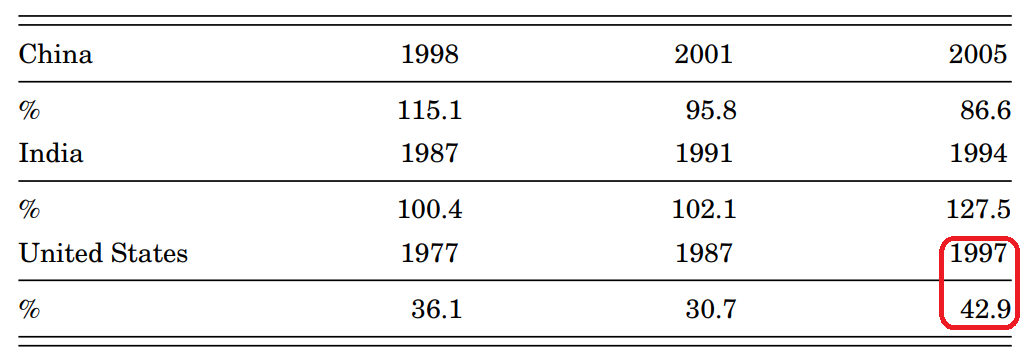
\includegraphics[width=0.8\linewidth]{Table 2 - TFP Gains.png}
      \end{table}
\end{frame}

\begin{frame}{Less Medium, More Extreme!}
    \begin{figure}
        \centering
            \begin{subfigure}[m]{0.45\textwidth}
                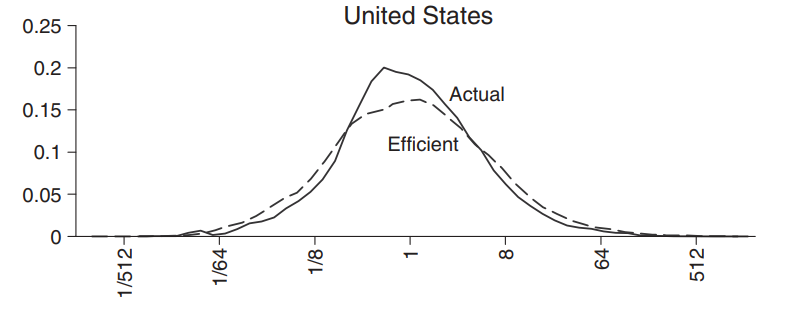
\includegraphics[width=1.05\textwidth]{US-Gain.png}
                \label{fig:sfig41}
            \end{subfigure}
            \hspace*{0.5cm}
            \begin{subfigure}[m]{0.45\textwidth}
                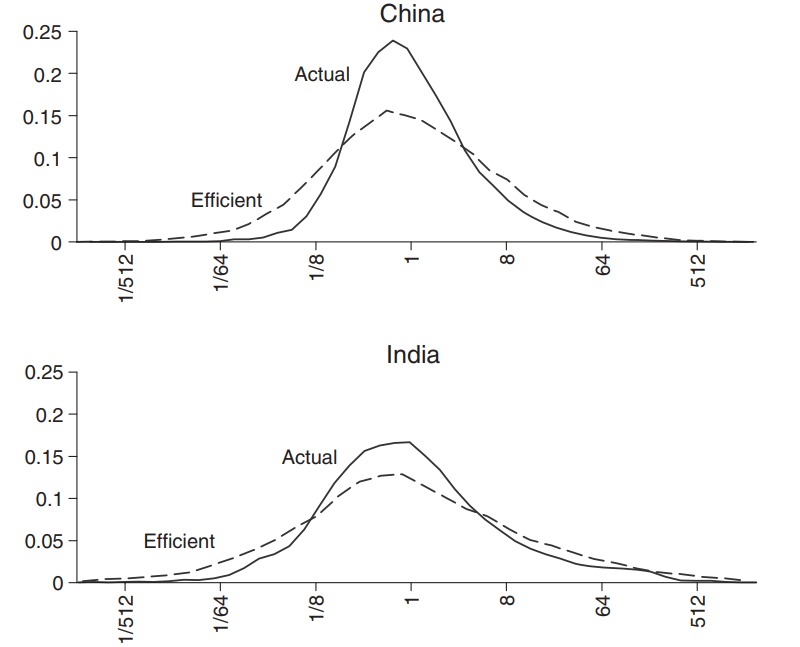
\includegraphics[width=1.05\textwidth]{China-India Gain.png}
                \label{fig:sfig42}
            \end{subfigure}
        \caption{Distribution of Plant Size}
        \label{fig:fig4}
        \end{figure}  
\end{frame}
\begin{frame}{As Productive as the Worst US!}
    \begin{table}
        \caption{TFP Gains from Equalizing TFPR realtive to 1997 U.S. gains}
        \label{tbl:tbl2}
        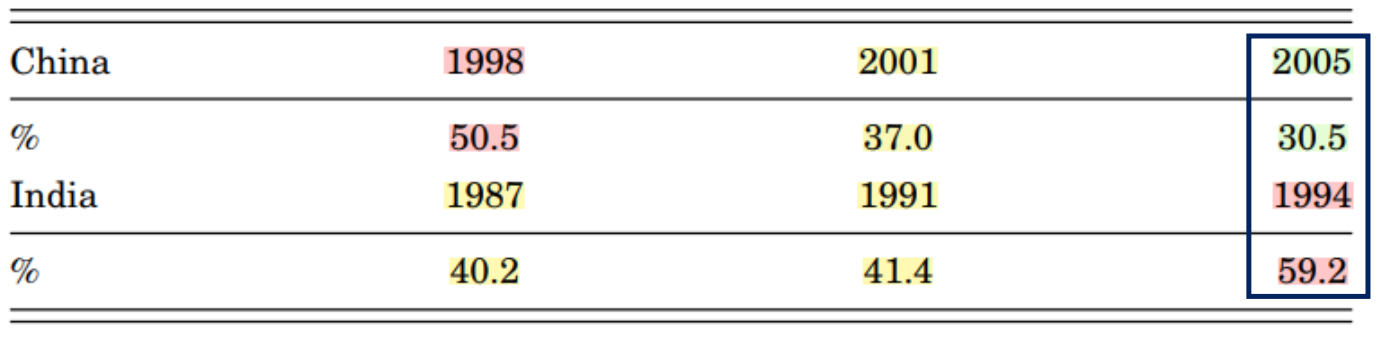
\includegraphics[width=0.8\linewidth]{Comapre to US.png}
      \end{table}
\end{frame}
\begin{frame}{The Virtuous Cycle of TFP-Output}
            \begin{itemize}
                \onslide<1-2>\item Capital accumulation significantly amplifies the impact of TFP gains on manufacturing output.
                \onslide<2-2>\item A 30\% increase in TFP in China, could result in 69\% increase in manufacturing output.
                \onslide<2-2>\item A 59\% increase in TFP in India, could result in 153\% increase in manufacturing output.
            \end{itemize}
\end{frame}
\begin{frame}{TFPR Distribution}
    \begin{figure}
        \centering
            \begin{subfigure}[m]{0.45\textwidth}
                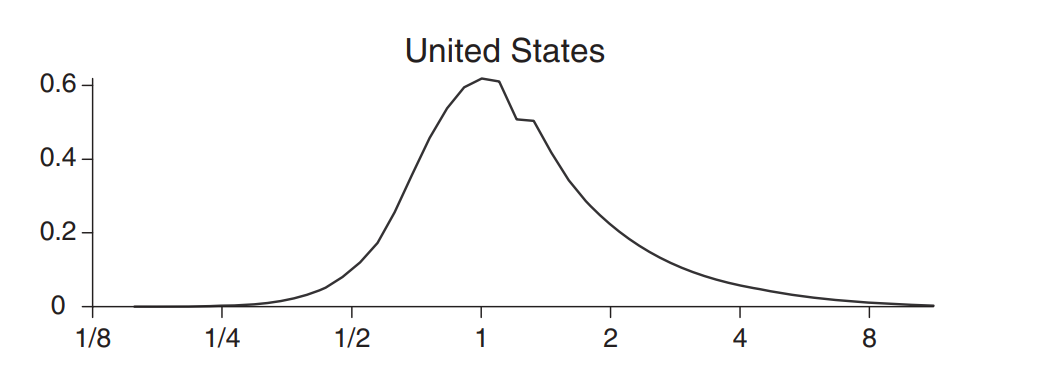
\includegraphics[width=1.1\textwidth]{US-TFPR.png}
                \label{fig:sfig21}
            \end{subfigure}
            \hspace*{0.5cm}
            \begin{subfigure}[m]{0.45\textwidth}
                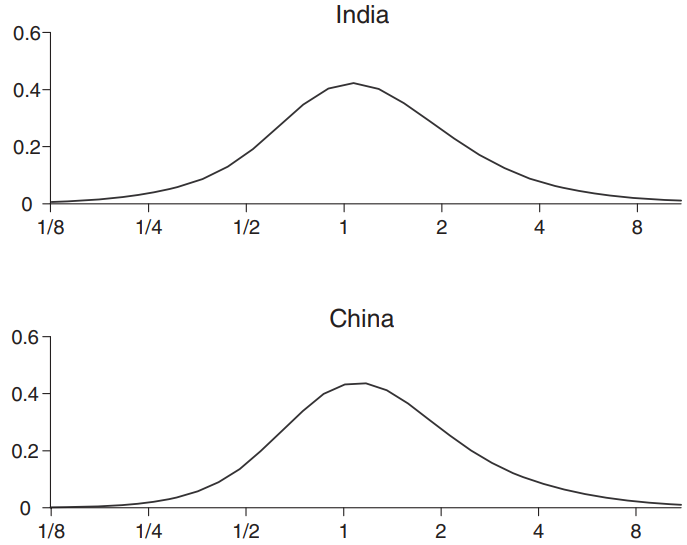
\includegraphics[width=1.05\textwidth]{China-India TFPR.png}
                \label{fig:sfig22}
            \end{subfigure}
        \caption{Distribution of TFPR}
        \label{fig:fig2}
        \end{figure}  
\end{frame}

\begin{frame}{TFPQ Distribution}
    \begin{figure}
        \centering
            \begin{subfigure}[m]{0.45\textwidth}
                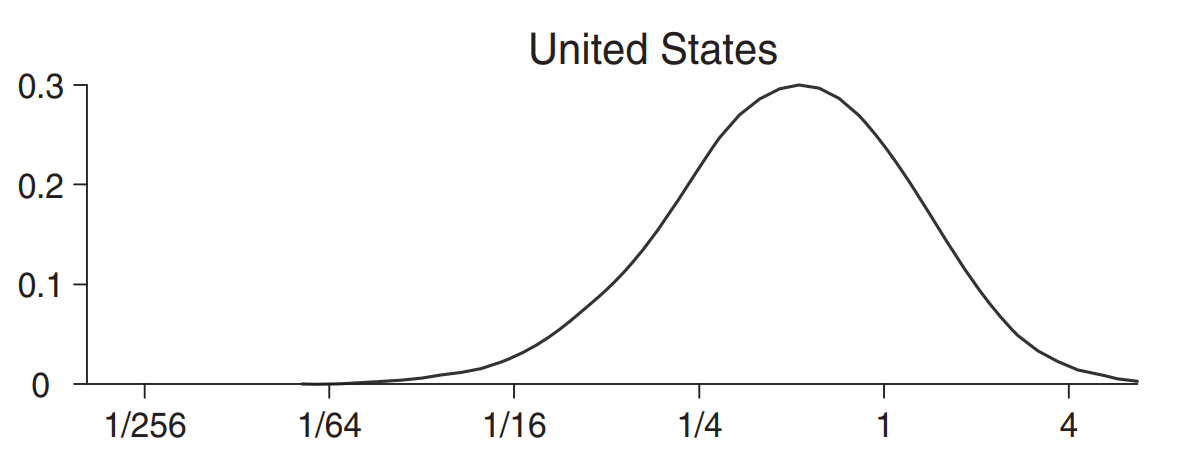
\includegraphics[width=1.05\textwidth]{US-TFPQ.png}
                \label{fig:sfig11}
            \end{subfigure}
            \hspace*{0.5cm}
            \begin{subfigure}[m]{0.45\textwidth}
                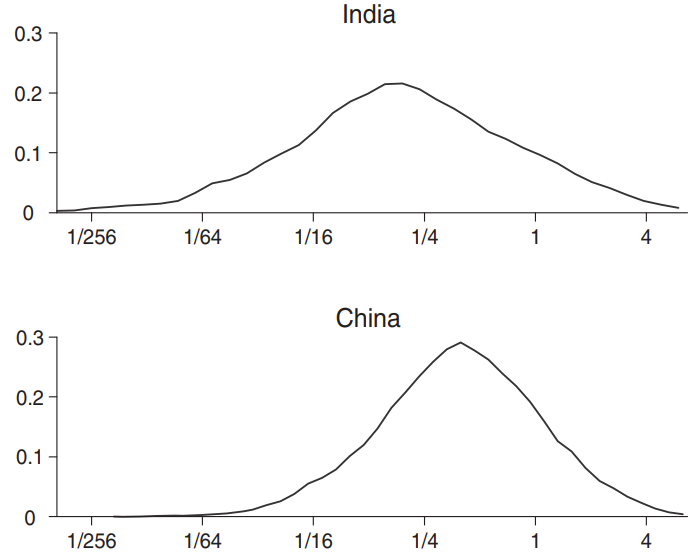
\includegraphics[width=1.05\textwidth]{China-India TFPQ.png}
                \label{fig:sfig12}
            \end{subfigure}
        \caption{Distribution of TFPQ}
        \label{fig:fig1}
        \end{figure}  
\end{frame}

\begin{frame}{Revealing the Enigma: TFPR in China}
    \begin{itemize}
        \item The state-owned plants in China decreased from 29\% in 1998 to 8\% in 2005.
        \item SOE in China had 40\% lower TFPR compared to private domestic plants. 
    \end{itemize}
    \begin{table}
        \caption{Regressions of Sector TFPR Dispersion on State Ownership in China}
        \label{tbl:tbl3}
        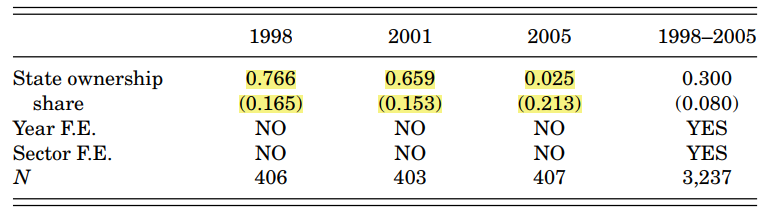
\includegraphics[width=0.8\linewidth]{TFPR reg - china.png}
      \end{table}
\end{frame}

\begin{frame}{Revealing the Enigma: TFPR in India}
    \begin{table}
        \captionsetup{justification=centering}
        \caption{Regression of Sector TFPR Dispression on Delicensing and Size Restrictions in India}
        \label{tbl:tbl4}
        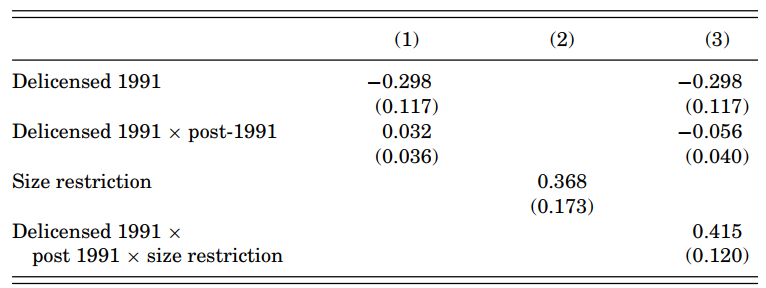
\includegraphics[width=0.8\linewidth]{TFPR reg - India.png}
      \end{table}
\end{frame}

\section{Conclusion}
\begin{frame}{Conclusion}
    \begin{itemize}
        \onslide<1-3>\item The study examined misallocation of inputs in manufacturing plants in China (1998–2005) and India (1987–1994) compared to the United States (1977, 1987, 1997).
        \onslide<2-3>\item Analysis revealed larger gaps in the marginal products of labor and capital across plants within industries in China and India compared to the United States.
        \onslide<3-3>\item Simulations indicated that aligning with U.S. dispersion of marginal products could significantly increase TFP in both China (30\%–50\% increase) and India (40\%–60\% increase).
    \end{itemize}
\end{frame}

\begin{frame}
    \centering
    \Huge{Thank You!}
\end{frame}
\end{document}

%%%%%%%%%%%%%%%%%%%%%%%%%%%%%%%%%%%%%%%
%%%%%%%%%%%%%%%%%%%%%%%%%%%%%%%%%%%%%%%

\begin{frame}{India:}
    \begin{itemize}
        \onslide<1-4>\item Data sourced from India's Annual Survey of Industries (ASI) conducted by the Central Statistical Organisation.
        \onslide<2-4>\item ASI covers registered manufacturing plants with over 50 workers and a random one-third sample of those with 10 to 50 workers.
        \onslide<3-4>\item Spans fiscal years from 1987-1988 to 1994-1995, encompassing approximately 40,000 plants annually.
        \onslide<4-4>\item Data includes industry classification, labor compensation, value-added, plant age, and capital.
    \end{itemize}
\end{frame}

\begin{frame}{China:}
    \begin{itemize}
        \onslide<1-5>\item Data sourced from China's Annual Surveys of Industrial Production, conducted by the government's National Bureau of Statistics.
        \onslide<2-5>\item Surveys encompass all non-state firms with over 5 million yuan in revenue plus state-owned firms.
        \onslide<3-5>\item Covering 1998 to 2005. Initially over 100,000 firms in 1998, growing to 200,000+ by 2005.
        \onslide<4-5>\item Data includes industry classification, plant age, ownership, wages, value-added, exports, and capital.
        \onslide<5-5>\item Nonwage benefits are estimated to maintain a total of 50\% of value-added alongside reported wages.
    \end{itemize}
\end{frame}

\begin{frame}{United States:}
    \begin{itemize}
        \onslide<1-3>\item Data sourced from he Census of Manufactures (CM) from 1977, 1982, 1987, 1992, and 1997 conducted by the U.S. Bureau of the Census.
        \onslide<2-3>\item The census covers all manufacturing plants, excluding small plants with limited production data (Administrative Records), leaving 160,000+ plants per year.
        \onslide<3-3>\item Capital stock is calculated as the mean of year's start and end, while plant age is estimated based on its initial appearance in the dataset.
    \end{itemize}
\end{frame}

\begin{frame}{Results - TFPR}
    \begin{table}
        \caption{Percent Sources of TFPR Variation within Industries}
        \label{tbl:tbl1}
        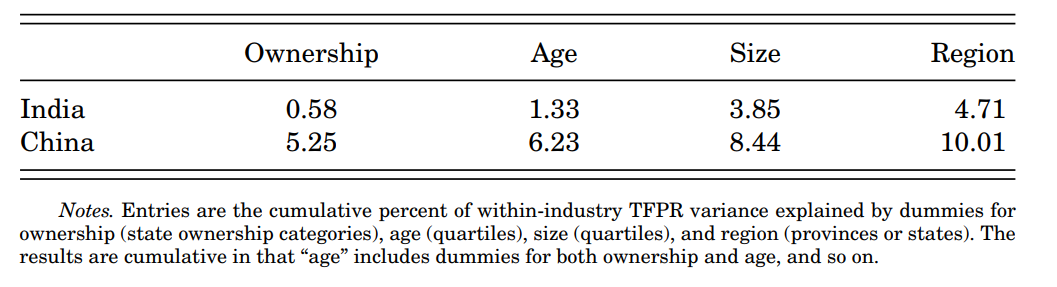
\includegraphics[width=0.9\linewidth]{Table 1.png}
      \end{table}
\end{frame}
\begin{frame}{The Menace of Misallocation}
    \begin{itemize}
            \onslide<1-2>\item Bosworth and Collins (2007) found China’s industry had 6.2\% annual TFP growth (1993-2004),
            (2\% from better resource allocation), while India’s TFP grew just 0.3\% annually (1978-1993) due to worsening allocations.
            \onslide<2-2>\item Resource misallocation may contribute to:
            \begin{itemize}
                \item 49\% of the TFP gap between the US and China.
                \item 35\% of the TFP gap between the US and India.
            \end{itemize}    
    \end{itemize}
\end{frame}

\section{Counter Factual}
\begin{frame}{A Utopian Economy!}
    \begin{itemize}
        \onslide<1-2>\item Aggregate TFPQ for a no-distortion industry:
        \begin{equation}
            \bar A_s = \left( \prod_{i=1}^{M_s} A_{si}^{\sigma-1} \right)^{\frac{1}{\sigma-1}}
        \end{equation}
        \onslide<2-2>\item Aggregate this ratio across sectors using our Cobb-Douglas
        aggregator \hyperref[eq:eqn1]{equation (1)}:
        \begin{equation}
            A_{si} = \kappa_s \cdot\dfrac{ (P_{si}Y_{si})^{\frac{\sigma}{\sigma - 1}}}{ K_{si}^{\alpha_s} \cdot L_{si}^{1 - \alpha_s}} \text{\;\;in which:\;\;} \kappa_s = \frac{w^{1 - \alpha_s} (P_s Y_s)^{-\frac{\sigma - 1}{\sigma}}}{P_s}
        \end{equation}
    \end{itemize}
\end{frame}

















